\documentclass[10pt,a4paper]{article}
\usepackage[utf8]{inputenc}
\usepackage[english]{babel}
\usepackage[T1]{fontenc}
\usepackage{amsmath}
\usepackage{amsfonts}
\usepackage{amssymb}
\usepackage{subcaption}
\usepackage{makeidx}
\usepackage{graphicx}
\usepackage{fourier}
\usepackage{listings}
\usepackage{color}
\usepackage{hyperref}
\usepackage[left=2cm,right=2cm,top=2cm,bottom=2cm]{geometry}
\author{Tommy Müller, Marcus Dittrich, Vincent Noculak}
\title{Zeeman-Effekt}


\begin{document}

\maketitle
\newpage
\tableofcontents
\newpage

\section{Durchführung}

\subsection{Eichkurve}

Die für den Versuch angezeigte Gleichspannung entsprach nicht der tatsächlich angelegten Spannung. Deshalb musste vor der Messung eine Eichkurve gemessen werden. Die gemessene Eichkurve ist in Abbildung \ref{eichkurve1} zu sehen. Es kann ein linearer Zusammenhang zwischen der abgelesenen und tatsächlich angelegten Spannung erkannt werden. Mit der Methode der kleinsten Quadrate wurde eine Ausgleichsgerade durch die Messwerte gelegt. Mit dieser Methode wurde auch der Fehler der Steigung der Gerade abgeschätzt. Die Steigung der Ausgleichsgerade beträgt $0,0824 \pm 0,0002$. Wegen dem linearen Zusammenhang muss beim Ablesen einer Spannung diese nur mit der Steigung der Ausgleichsgerade multipliziert werden, um die angelegte Spannung zu berechnen.

\begin{figure}[h]
	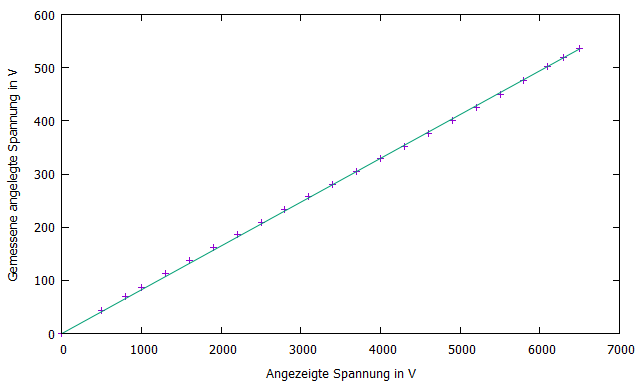
\includegraphics[scale = 0.7]{eichkurve.png}
	\centering
	\caption{Eichkurve der angelegten Gleichspannung; Steigung der Ausgleichsgerade: $0,0824 \pm 0,0002$}
	\label{eichkurve1}
\end{figure}

\end{document}